% Figure: DeltaSort worst-case movement diagram
\begin{figure}
\centering
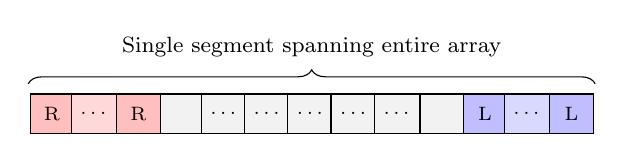
\begin{tikzpicture}[
    cell/.style={minimum width=0.55cm, minimum height=0.5cm, draw, font=\scriptsize, outer sep=0pt},
    dotcell/.style={minimum width=0.55cm, minimum height=0.5cm, draw, font=\scriptsize, outer sep=0pt},
    right/.style={cell, fill=red!25},
    left/.style={cell, fill=blue!25},
    clean/.style={cell, fill=gray!10, font=\scriptsize},
    segbrace/.style={decorate, decoration={brace, amplitude=5pt}},
    seglabel/.style={font=\footnotesize},
    movearrow/.style={->, thick, >=stealth},
    rmovelabel/.style={font=\scriptsize, text=red!70!black},
    lmovelabel/.style={font=\scriptsize, text=blue!70!black}
]

% Array position
\def\yarr{0}
\def\ymove{-1.0}
\def\cellw{0.55}

% === R CLUSTER (all R-direction updates at the start) ===
\node[right] (r1) at (0, \yarr) {R};
\node[dotcell, fill=red!15] at (\cellw, \yarr) {\dots};
\node[right] (r2) at (2*\cellw, \yarr) {R};

% === LARGE CLEAN REGION (unchanged values) ===
\node[clean] (c1) at (3*\cellw, \yarr) {};
\node[dotcell, fill=gray!10] at (4*\cellw, \yarr) {\dots};
\node[dotcell, fill=gray!10] at (5*\cellw, \yarr) {\dots};
\node[dotcell, fill=gray!10] at (6*\cellw, \yarr) {\dots};
\node[dotcell, fill=gray!10] at (7*\cellw, \yarr) {\dots};
\node[dotcell, fill=gray!10] at (8*\cellw, \yarr) {\dots};
\node[clean] (c2) at (9*\cellw, \yarr) {};

% === L CLUSTER (all L-direction updates at the end) ===
\node[left] (l1) at (10*\cellw, \yarr) {L};
\node[dotcell, fill=blue!15] at (11*\cellw, \yarr) {\dots};
\node[left] (l2) at (12*\cellw, \yarr) {L};

% === SINGLE SEGMENT BRACE (top) ===
\draw[segbrace] (-0.3, 0.38) -- (12*\cellw+0.3, 0.38);
\node[seglabel] at (6*\cellw, 0.85) {Single segment spanning entire array};


\end{tikzpicture}
\caption{Worst-case configuration for DeltaSort. This occurs when updated values monotonically cluster at the start and end of the array, forming a single segment that spans the entire array. }
\label{fig:worst-case}
\end{figure}
